\chapter{Evaluation}
\label{ch:evaluation}
The evaluation chapter describes the experimental setup, the data set and the results.

\section{Data Set}
\label{sec:dataset}
The data set consists of data from the Flickr API \footnote{\url{https://www.flickr.com/services/api/}}.
Flicker provides an API endpoint which contains data of the latest posted images.
As the API limits the number of requests per hour, the data had to be collected over an extended period of time.
The test data were gathered from this endpoint over a time period of about 4 weeks.

The internal representation in Elasticsearch of the data from Flickr can be seen in appendix \ref{ap:flickr-data}.
This data contains 115,105 photos and 298,962 tags, and the photo index takes up 152.3 MB in Elasticsearch.
Dynamic mapping was used for defining the fields for the internal representation in Elasticsearch.
A single index called \textit{photos} was used to hold the photo data.

\section{Experimental Setup}
The experimental setup consists of two main parts, a client and a web server.
A laptop was used as the client and a desktop as the web server.
Both computers were placed on the same local network.
The hardware specification of the laptop was: Intel Core i7 2.50 GHz x 4 and 8 GB DDR3L RAM,
and the desktop had the following specifications: Intel Core i5 3.40 GHz x 4 and 16 GB of DDR3 RAM.

The web server contained both Elasticsearch and the NodeJS web server.
Elasticsearch's configuration was set to default settings,
except that the memory heap size was changed from the default value of 2 GB to 4 GB.
Elasticsearch v5.0.0 was used during the experiment.

As mentioned earlier NodeJS was configured to use the internal clustering functionality.
Using a desktop with 4 cores, the web server was running 4 instances of NodeJS.
NodeJS accessed Elasticsearch through the available HTTP REST API \cite{elasticsearch-rest-api}.

\subsection{Performance Metrics}
The performance metric used in this experiment was latency.
Latency was measured from when the request left the laptop to the response was retrieved.
The command line tool called \texttt{ab} \cite{apache-benchmark} was used to evaluate the latency.


%Figure \ref{fig:experiment-setup} illustrates the experiment setup.
%\begin{figure}[h!]
%  \centering \includegraphics[width=0.9\linewidth]{img/experiment_setup.png}
%  \caption{Experiment setup}
%  \label{fig:experiment-setup}
%\end{figure}

%\begin{table}[h]
%    \centering
%    \begin{tabular}{c|c}
%      \textbf{Component} & \textbf{Model} \\ \hline
%      CPU       & Intel Core i5-4670 3.4 GHz x 4        \\ \hline
%      RAM       & Crucial BallistixSport 2x8GB 1600 MHz \\ \hline
%      SSD       & OCZ Vertex 4 256 GB                   \\ \hline
%    \end{tabular}
%    \caption{Hardware components of the computer running the experiments}
%    \label{tbl:hardware}
%\end{table}

\section{Results}
\label{sec:results}
Elasticsearch caches frequently used aggregations.
To utilize this feature of Elasticsearch the same query was sent each time.
The query contained the top 5 most popular tags from the data set: \textit{"square", "iphoneography", "squareformat", "instagramapp", "uploaded:by=instagram"}.
Each request was sent 1000 times, and the average and median latency were calculated.

Three different types of tests were conducted: query without expansion, query with expansion, and a query where the number of top-k documents varied.
The first two tests varied the number of concurrent requests from 1 to 150.
The last test had a fixed number of concurrent request at 10,
but varied the number of top-k documents from 10 to 200.

To measure the impact of query expansion a baseline is needed.
The baseline results were retrieved by using the same terms but withouth the query expansion.
Table \ref{tbl:baseline} displays results from the baseline test.
From the table we can see that the backend was able to handle between 50 and 100 concurrent requests and still meet the interactivity requirement.

The test results from the requests with query expansion are listed in table \ref{tbl:query-expansion}.
In the table one can see that query expansion has a clear impact on the latency, even with only one concurrent request.
However, the query expansion implementation is able to meet the interactivity with up to 20 concurrent requests.
Compared to the results from the baseline,
the query expansion implementation is able to handle less than half the number of requests.

On the last test the number of top-k documents varied and the results are listed in table \ref{tbl:query-expansion-topk}.
To make sure the web server was not the bottleneck, the number of concurrent requests were fixed at 10.
As \texttt{k} increases from 10 to 200, the latency increased.
From the table one can see that varying the \texttt{k} has little impact on the performance.
The latency increased from below 50 ms to between 70 and 80 ms, which is still within the interactivity requirement.
The increased latency is most likely due to the query expansion step on the web server,
the increased data size from Elasticsearch and from Elasticsearch itself.

\begin{table}[h]
    \centering
    \begin{tabular}{c|l|l}
    Concurrent requests & Average (ms) & Median (ms) \\ \hline
    1                   & 8            & 7           \\ \hline
    5                   & 13           & 13          \\ \hline
    10                  & 20           & 20          \\ \hline
    15                  & 28           & 28          \\ \hline
    20                  & 34           & 35          \\ \hline
    30                  & 49           & 50          \\ \hline
    40                  & 63           & 63          \\ \hline
    \textbf{50}         & \textbf{73}  & \textbf{74} \\ \hline
    100                 & 123          & 115         \\ \hline
    150                 & 260          & 226         \\ \hline
    \end{tabular}
    \caption{Response times without query expansion}
    \label{tbl:baseline}
\end{table}

\begin{table}[h]
    \centering
    \begin{tabular}{c|l|l}
     Concurrent requests & Average (ms) & Median (ms) \\ \hline
    1                    & 16           & 14          \\ \hline
    5                    & 29           & 28          \\ \hline
    10                   & 49           & 49          \\ \hline
    \textbf{15}          & \textbf{74}  & \textbf{69} \\ \hline
    \textbf{20}          & \textbf{97}  & \textbf{96} \\ \hline
    30                   & 183          & 199         \\ \hline
    40                   & 219          & 198         \\ \hline
    50                   & 249          & 242         \\ \hline
    100                  & 476          & 428         \\ \hline
    150                  & 731          & 717         \\ \hline
    \end{tabular}
    \caption{Response times with query expansion}
    \label{tbl:query-expansion}
\end{table}

\begin{table}[h]
    \centering
    \begin{tabular}{c|l|l}
     Number of top-k documents & Average (ms) & Median (ms) \\ \hline
    10                         & 49           & 49          \\ \hline
    15                         & 56           & 51          \\ \hline
    20                         & 54           & 53          \\ \hline
    30                         & 57           & 53          \\ \hline
    40                         & 57           & 54          \\ \hline
    50                         & 58           & 56          \\ \hline
    100                        & 64           & 62          \\ \hline
    200                        & 76           & 72          \\ \hline
    \end{tabular}
    \caption{Response times while changing number of top-k documents}
    \label{tbl:query-expansion-topk}
\end{table}


\section{Discussion}
Figure \ref{fig:sequence-diagram-search-master} shows the sequence diagram for Rudihagen's query expansion solution using KL.
From the figure we can see that 4 round trips are required from the web server, to the database and the search engine.
The implementation discussed in Chapter \ref{ch:approach} describes a solution to decrease the number of round trips from 4 to 2.
Even though the new implementation is able to cut the number of round trips in half, the same degree is not used.
Rudihagen used a search where the same query may return two different results for two different users.
The implemented query expansion in this report will always return the same results for the same query, given that the data set is equal.

Comparing table \ref{tbl:baseline} with \ref{tbl:query-expansion} we can see that the baseline delivers more than doble the number of concurrent requests.
From the sequence diagrams in figure \ref{fig:sequence-diagram-search} and in figure \ref{fig:sequence-diagram-search-baseline} we see that the difference is the extra post processing steps.
As a result, we can assume that most of the extra latency is mostly due to the extra query to Elasticsearch.

In side table \ref{tbl:baseline} and \ref{tbl:query-expansion} all the results within the interactivity limit are in bold.
The results from query expansion shows that 20 concurrent requests are within the requirement for interactivity.
However, these results are done in an environment were all the client and the server were on the same network,
and the web server and search engine were on the same physical machine.
In a real world application the web server and search engine would be on different machines,
resulting in significantly higher latencies.

\begin{figure}[h!]
\centering 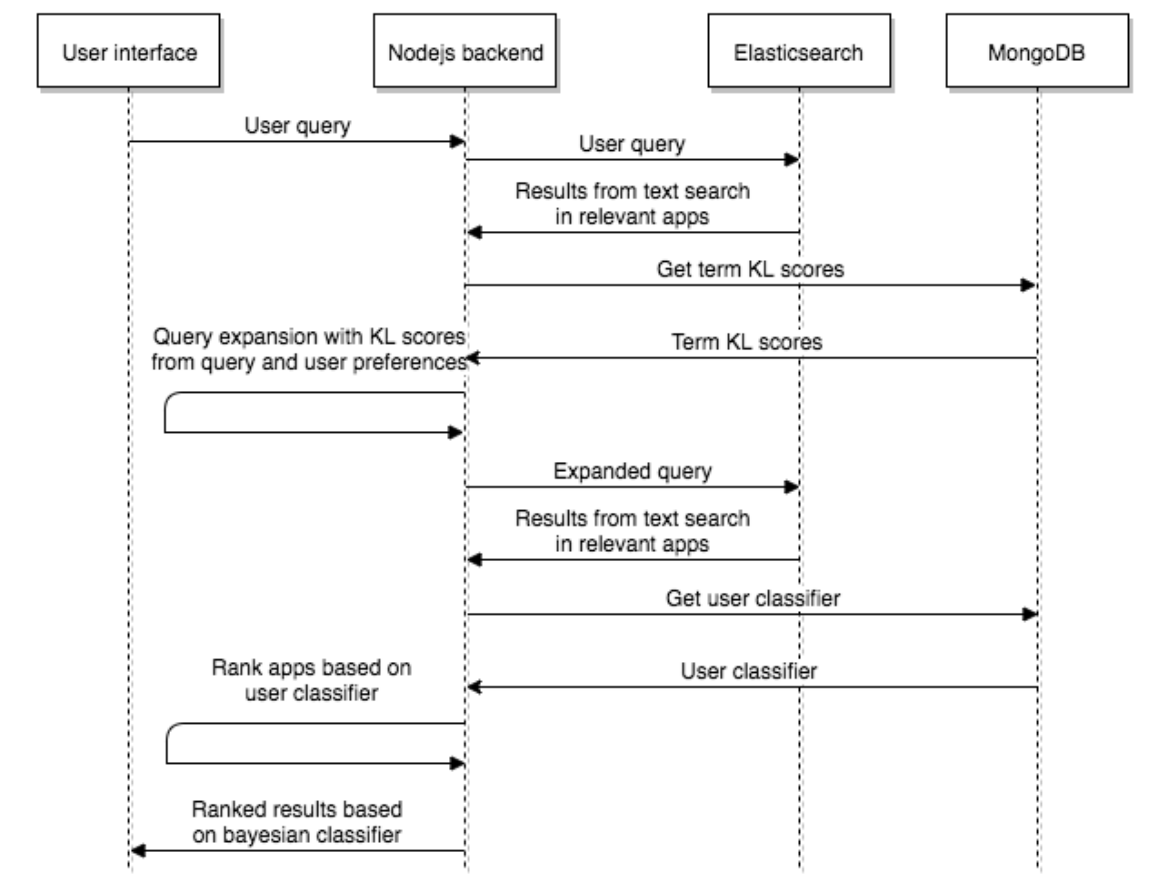
\includegraphics[width=0.9\linewidth]{img/sequence-diagram-search-master-thesis.png}
\caption{Sequence diagram from Rudihagen's master thesis implementation of query expansion using KL \cite[p. 37]{master-thesis}.}
\label{fig:sequence-diagram-search-master}
\end{figure}

Even though the latency was greatly reduced, there are a few disclaimers.
Firstly, both the webserver and the search engine ran on the same computer.
As a result the round trip time was almost negligible, which is often not the case in a real world environment.
To give more realistic measurements, the solution should be tested on a cloud solution where the web server and the search engine run on different physical servers.

\subsection{Evaluate Research Questions}
The following bulletpoints contains a discussion of the research questions from chapter \ref{ch:introduction}.

\begin{enumerate}
  %\item How to provide instant personalized recommendations on a cold start based on the query typed?
  \item \textbf{How to achieve more relevant search results based on a query from a user?} \newline
  As mentioned in section \ref{sec:problem-specification} the main focus areas were scaling and latency.
  Therefore, the relevance was never measured.
  Based on the work by Rudihagen,
  this project report assumes that query expansion returns more relevant results compared to the baseline search.

  \item\label{rq:scaling} \textbf{How to make the search recommandation scale with an increasing amount of data?} \newline
  As mentioned earlier, Elasticsearch is proven to scale to petabytes of data \cite{elasticsearch-scale},
  if configured correctly, and was thus used as the search engine for this project report.
  Rudihagen's implementation also used Elasticsearch, and was configured with one index for each user.
  This configuration is fine for most cases, but according to the documentation this does not scale well if you have a large user base \cite{elasticsearch-indices}.
  In the implementation a single index for the photos were used and 3 shards.
  If the data set had been larger the number of shardes should have been changed,
  but except for the shard configuration, the setup would be able to scale to large amounts of photo data.

  \item\label{rq:latency} \textbf{How to develop a search recommendation method that fulfills the interactive requirements?} \newline
  From the results we can see that the implementation is within the interactivity requirement of 100 ms, delivering results within 16 ms on average, given one concurrent request.
  The implementation is able to fullfill the interactivity requirement with up to 20 concurrent requests.
\end{enumerate}
